\documentclass[../Main.tex]{subfiles}
\begin{document}

%--------------------- Descripción del prototipo web ---------------------
\section{Descripción del prototipo web}
    \begin{justify}
    En esta sección se presenta el prototipo web de manera global, el cual cuenta con cinco (5) módulos principales, generación, examen, estadísticas, calificaciones y usuarios.
    
    El prototipo web está divido en dos tipos de perfiles, docente y estudiante. El perfil docente es donde se encuentran la mayor parte de módulos debido a la orientación de la solución, este cuenta con los cinco módulos anteriormente mencionados, mientras que el perfil estudiante cuenta con tres (3) de los cinco (5) módulos.
    
    En las siguientes secciones se describe cada módulo y submódulos con funcionalidades que puede realizar cada perfil, además, se describe y se presenta la interfaz gráfica de usuario.
    \end{justify}
    
\newpage
    %--------------------- Interfaz de usuario ---------------------
    \subsection{Interfaz de usuario}
    \begin{justify}
    Para la interfaz gráfica de usuario se comenzó con el diseño de un prototipo basado en las necesidades identificadas en la fase de análisis. Se utilizó la plataforma Figma la cual es una herramienta de generación de prototipos, el resultado se encuentra en los anexos.
    
    Como se mencionó en la sección 5.2 el prototipo web está compuesto por dos tipos de perfiles, el perfil docente tiene los módulos de generación, examen, calificaciones, estadísticas y usuarios (ajustes de cuenta), entre tanto, el perfil estudiante tiene los módulos examen, calificaciones y usuarios (ajustes de cuenta).
    %A continuación se muestra una imagen del perfil docente y estudiante respectivamente.
    \end{justify}
    
    \begin{figure}[H]
	\begin{Center}
		
\includegraphics[width=6.4in,height=3.3in]{Images/ui_homepage.png}
	    \caption{UI Homepage}
	    Fuente: Elaboración propia
        \label{fig:section}
	\end{Center}
    \end{figure}
    
\newpage    %--------------------- Usuarios del prototipo web ---------------------
    \subsection{Usuarios}
    \begin{justify}
    Este módulo contiene toda la información de los usuarios, realiza la gestión de los usuarios que se registran y de los usuarios que inician sesión, esta gestión permite visualizar y modificar la información personal del usuario.  
    \end{justify}
    
    \begin{figure}[H]
	\begin{Center}
		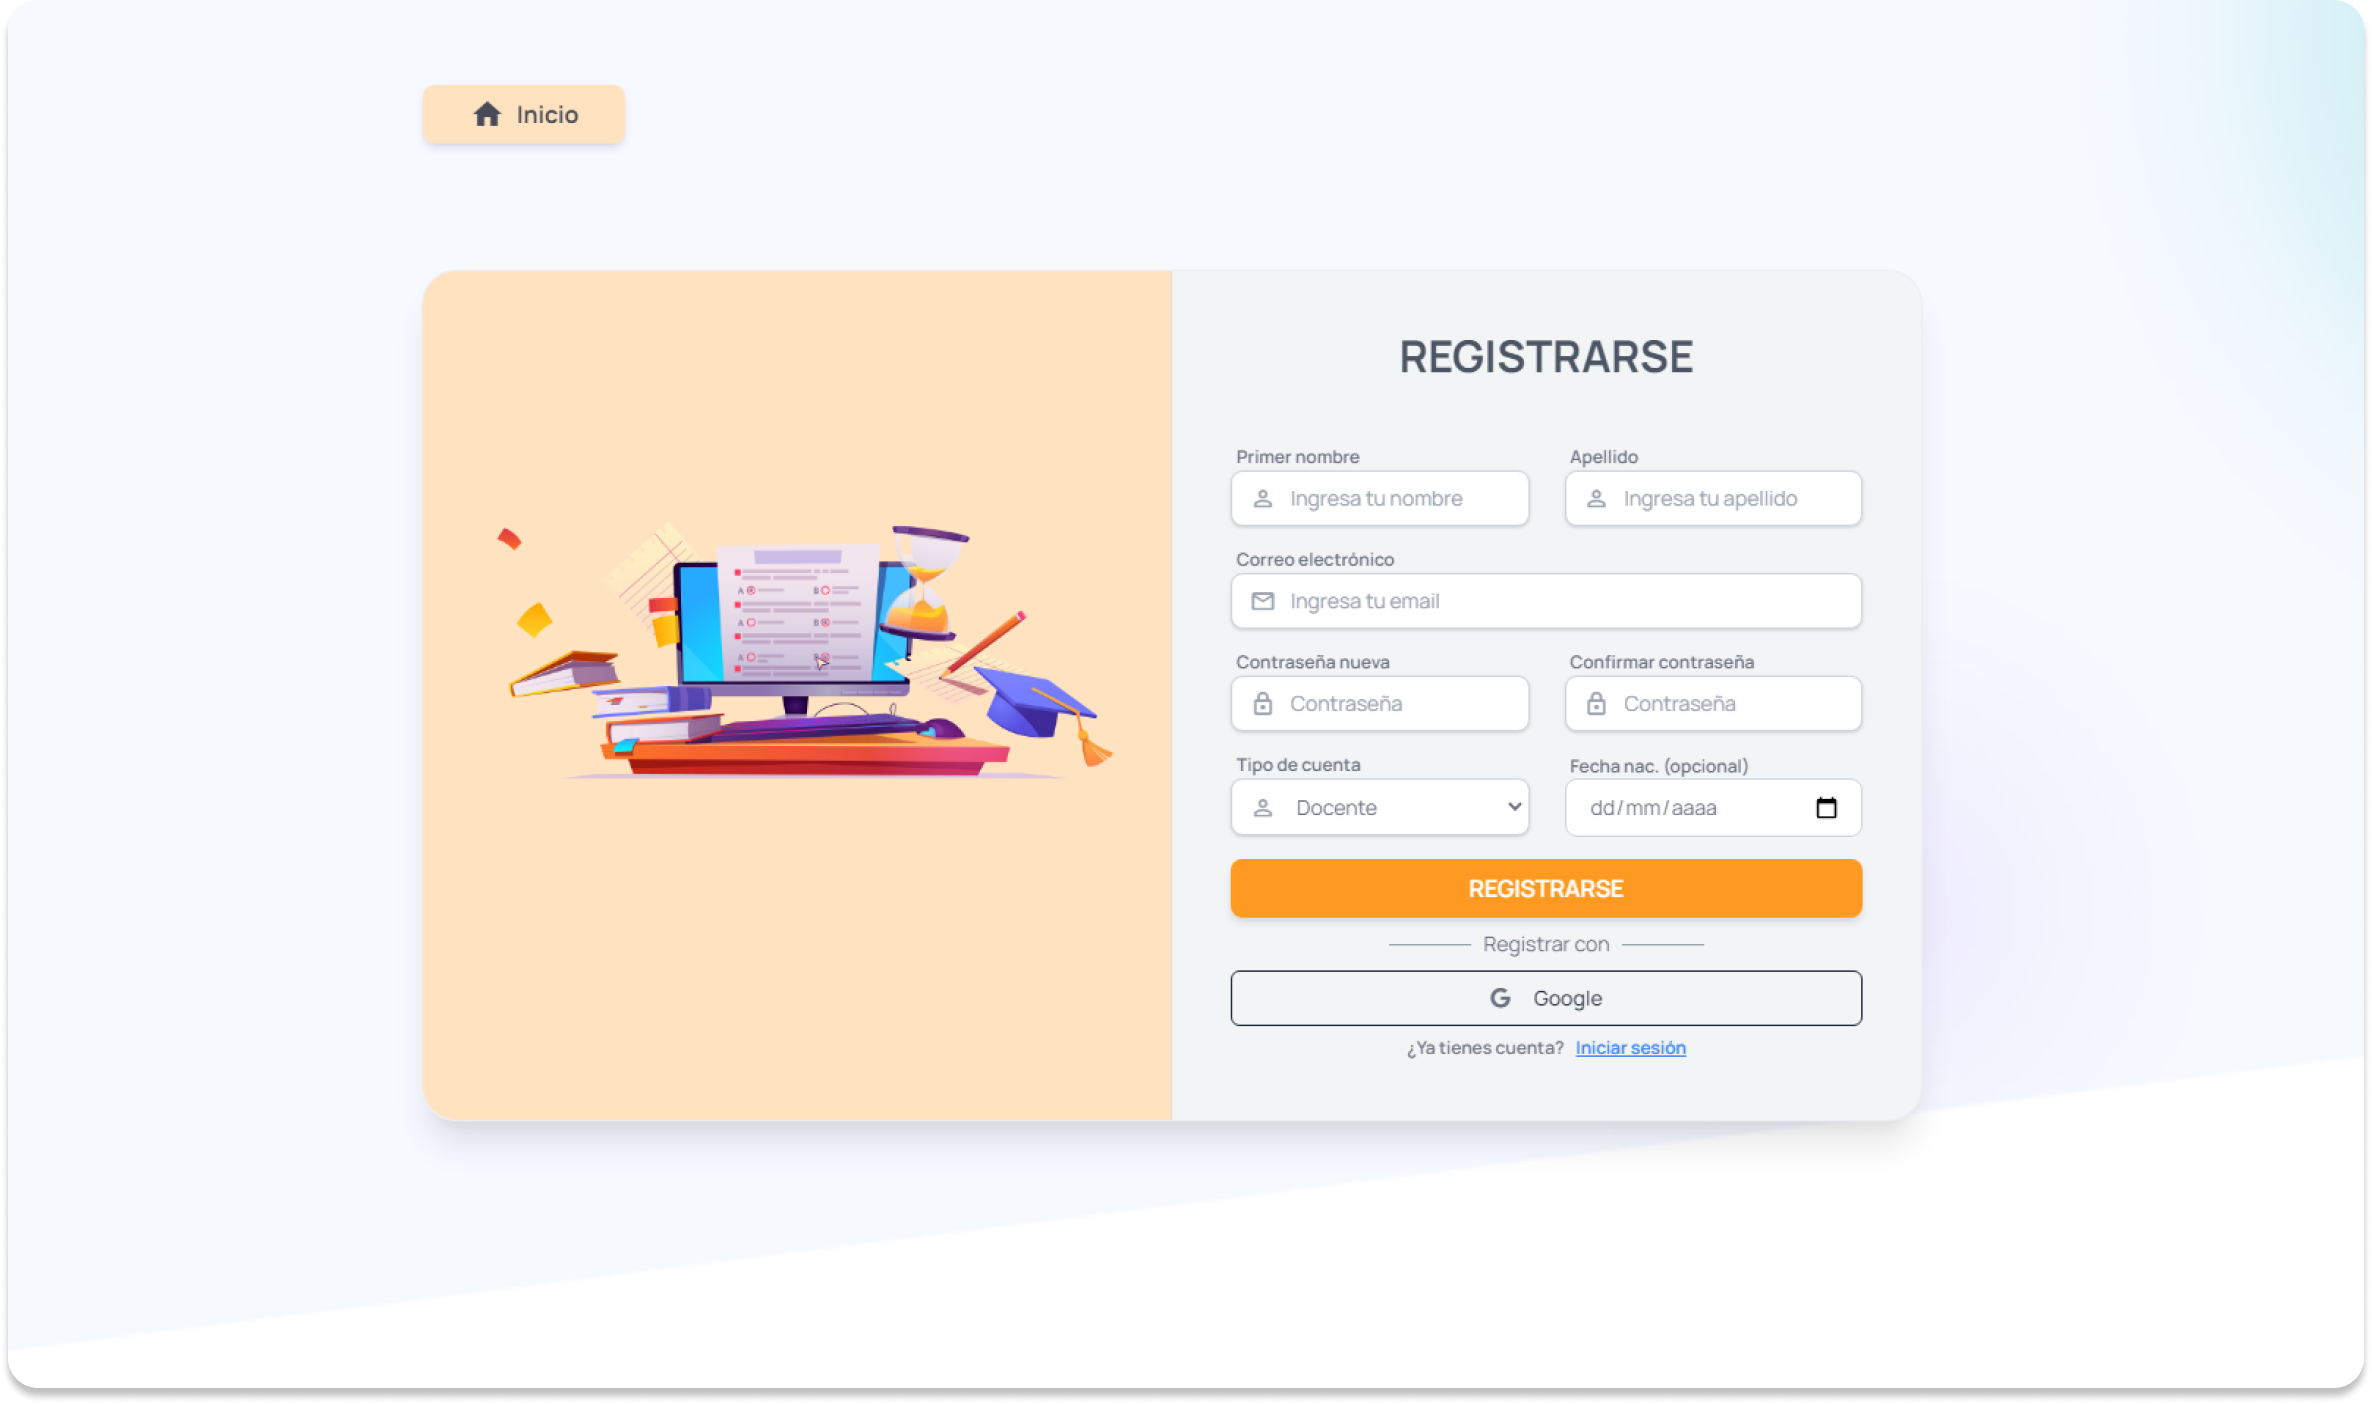
\includegraphics[width=6.4in,height=3.3in]{Images/ui_usuario_registro.png}
	    \caption{UI Registro de usuarios}
	    Fuente: Elaboración propia
        \label{fig:section}
	\end{Center}
    \end{figure}
    
    \begin{figure}[H]
	\begin{Center}
		
\includegraphics[width=6.4in,height=3.3in]{Images/ui_usuario_inicio_sesion.png}
	    \caption{UI Inicio de sesión}
	    Fuente: Elaboración propia
        \label{fig:section}
	\end{Center}
    \end{figure}
    
    %\section{Módulo Ingreso al prototipo web}
    %\subsection{Submódulo Inicio de sesión}
    %\subsection{Submódulo Registro de usuario}
    
    %--------------------- Módulo de generación ---------------------
    \subsection{Módulo Generación}
    \begin{justify}
    Este módulo es el más importantes de GQuestions, contiene varios submódulos que permiten la generación de exámenes y que conforman tres series de pasos vistos en las siguientes secciones.\\
    La palabra generación de aquí en adelante se refiere a el conjunto de exámenes y se utiliza de manera indistinta.
    \end{justify}
    
    %--------------------- subMódulo parámetros de generación ---------------------
    \subsubsection{Submódulo Parámetros de Generación}
    \begin{justify}
    Este submódulo representa el primer paso de la generación, permite configurar los parámetros de la generación entre los que están: cantidad de exámenes, longitud de texto, cantidad de preguntas, tipos de preguntas y el área del texto a generar (ej. Machine learning).\\
    Se puede visualizar el tiempo de espera promedio que tarda la generación de acuerdo a la configuración del mismo.
    \end{justify}
    
    \begin{figure}[H]
	\begin{Center}
		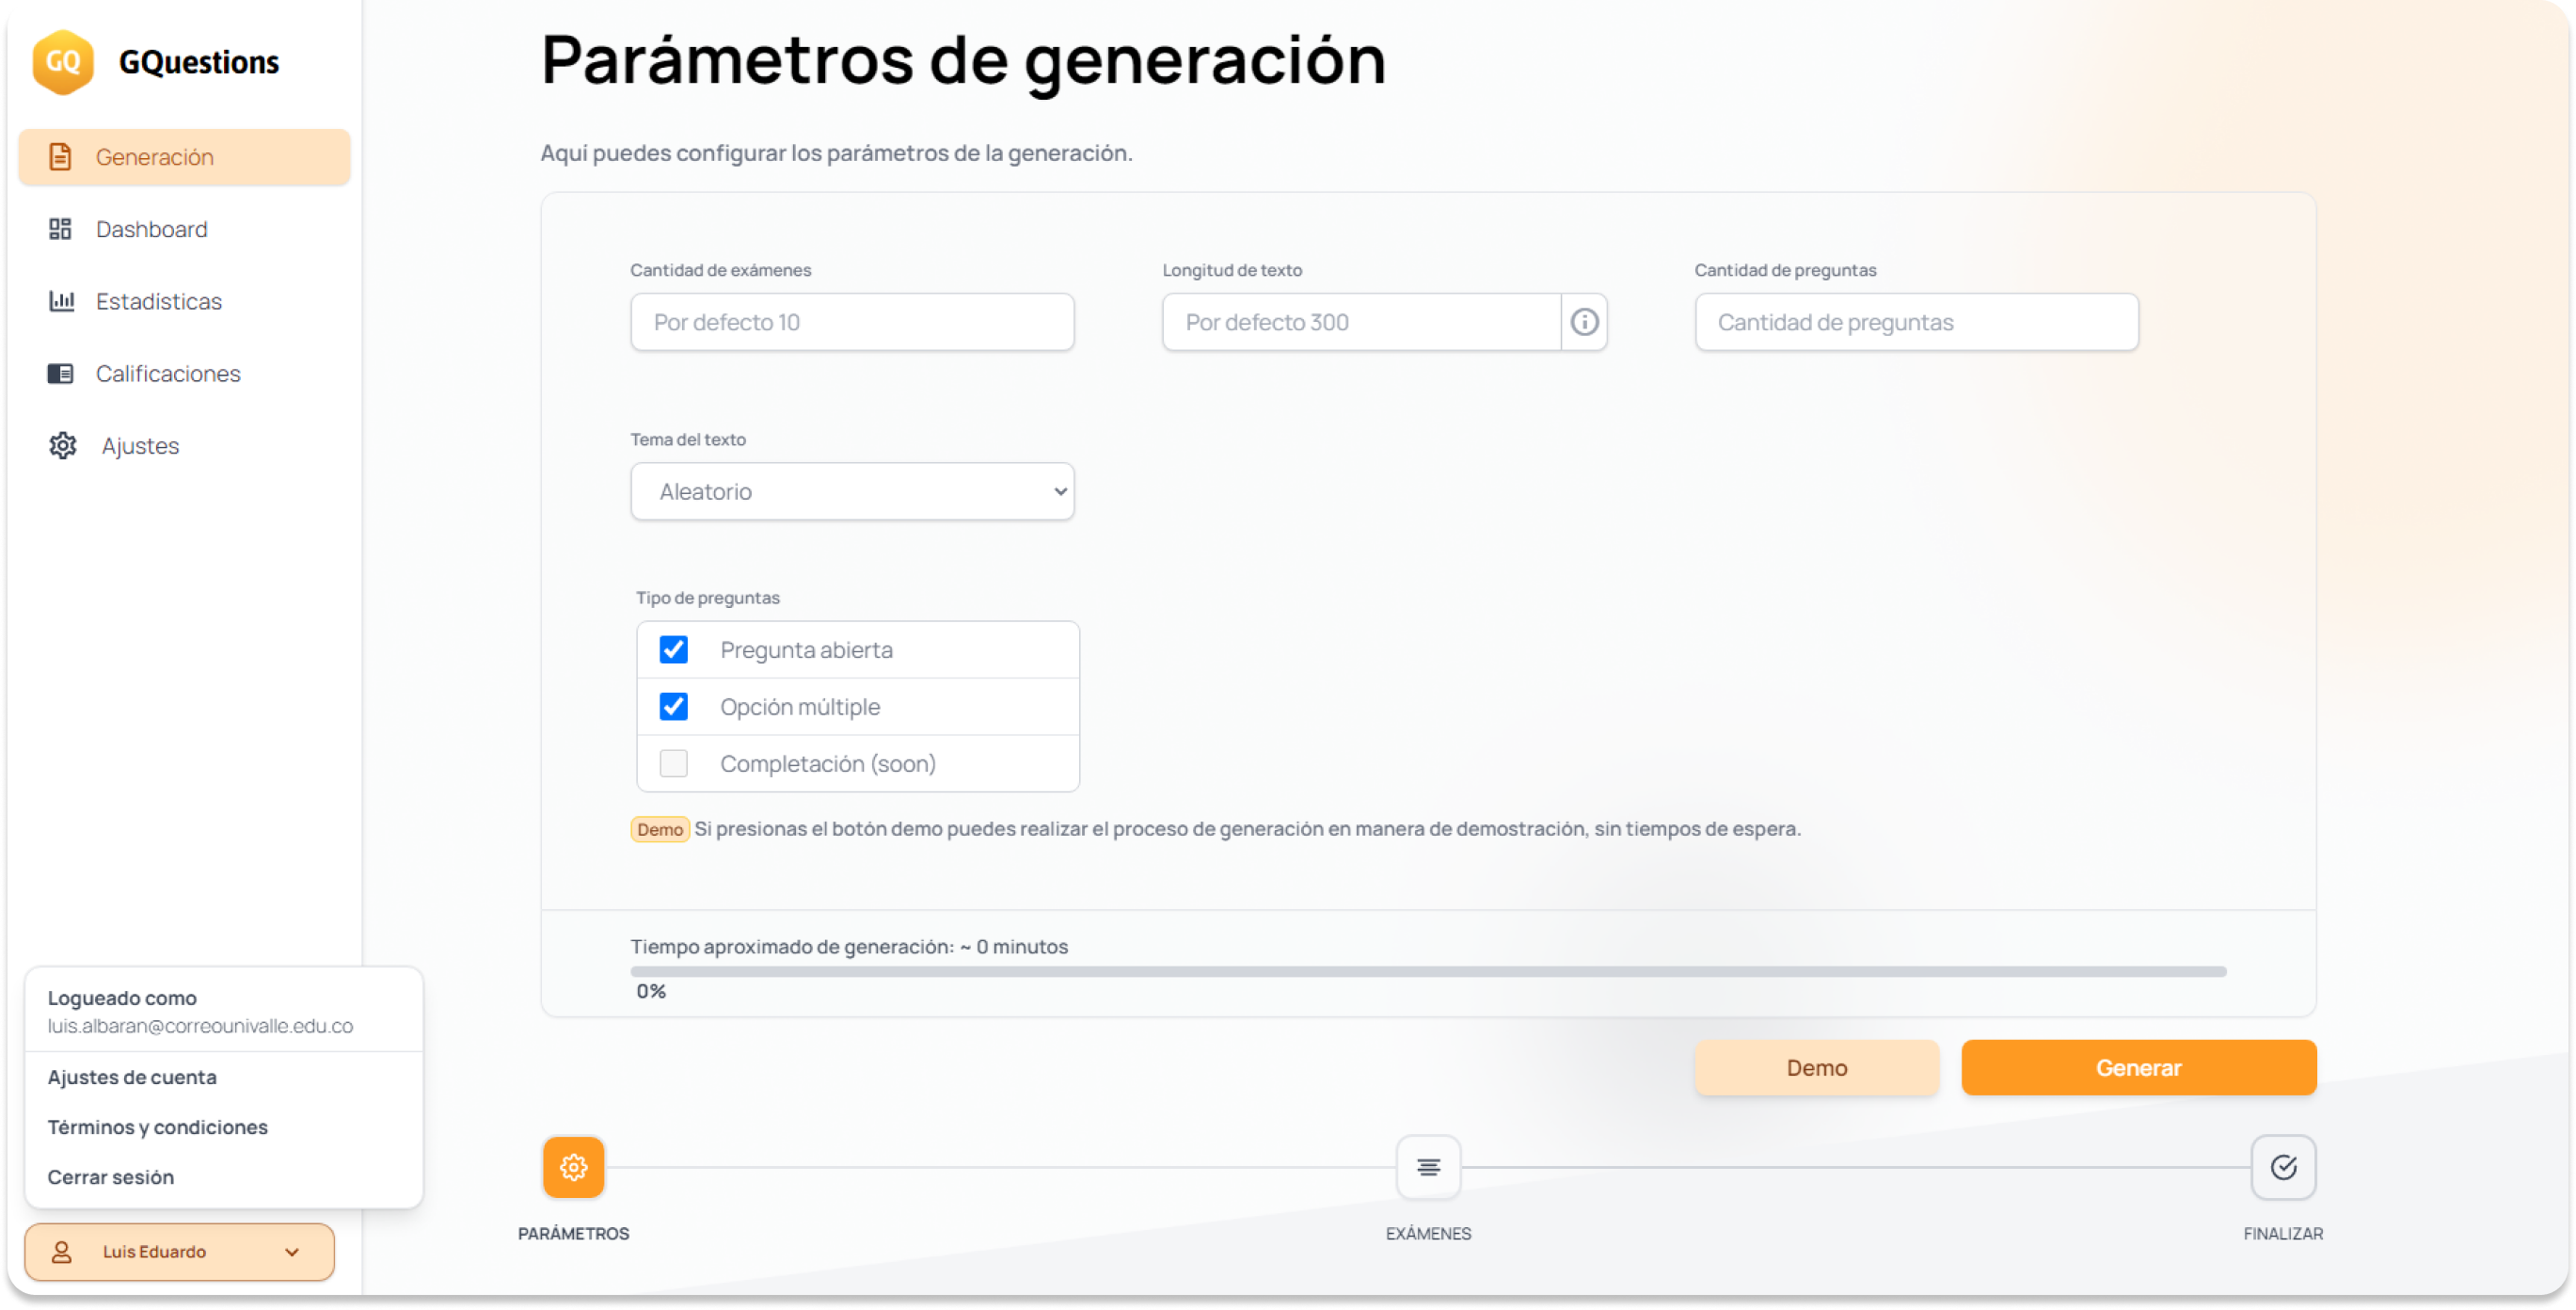
\includegraphics[width=6.4in,height=3.3in]{Images/ui_docente_generacion.png}
	    \caption{UI Párametros de generación - docente}
	    Fuente: Elaboración propia
        \label{fig:section}
	\end{Center}
    \end{figure}
    
    %------------------- subMódulo de revisión de generación ---------------------
    \subsubsection{Submódulo Revisión Generación}
    \begin{justify}
    Este submódulo representa el segundo paso de la generación, permite navegar por los exámenes generados, visualizar y modificar cada examen del conjunto, tanto texto base como preguntas generadas, además, permite volver a generar cualquier texto con sus preguntas en caso de no ser adecuado para el docente.
    \end{justify}
    
    \begin{figure}[H]
	\begin{Center}
		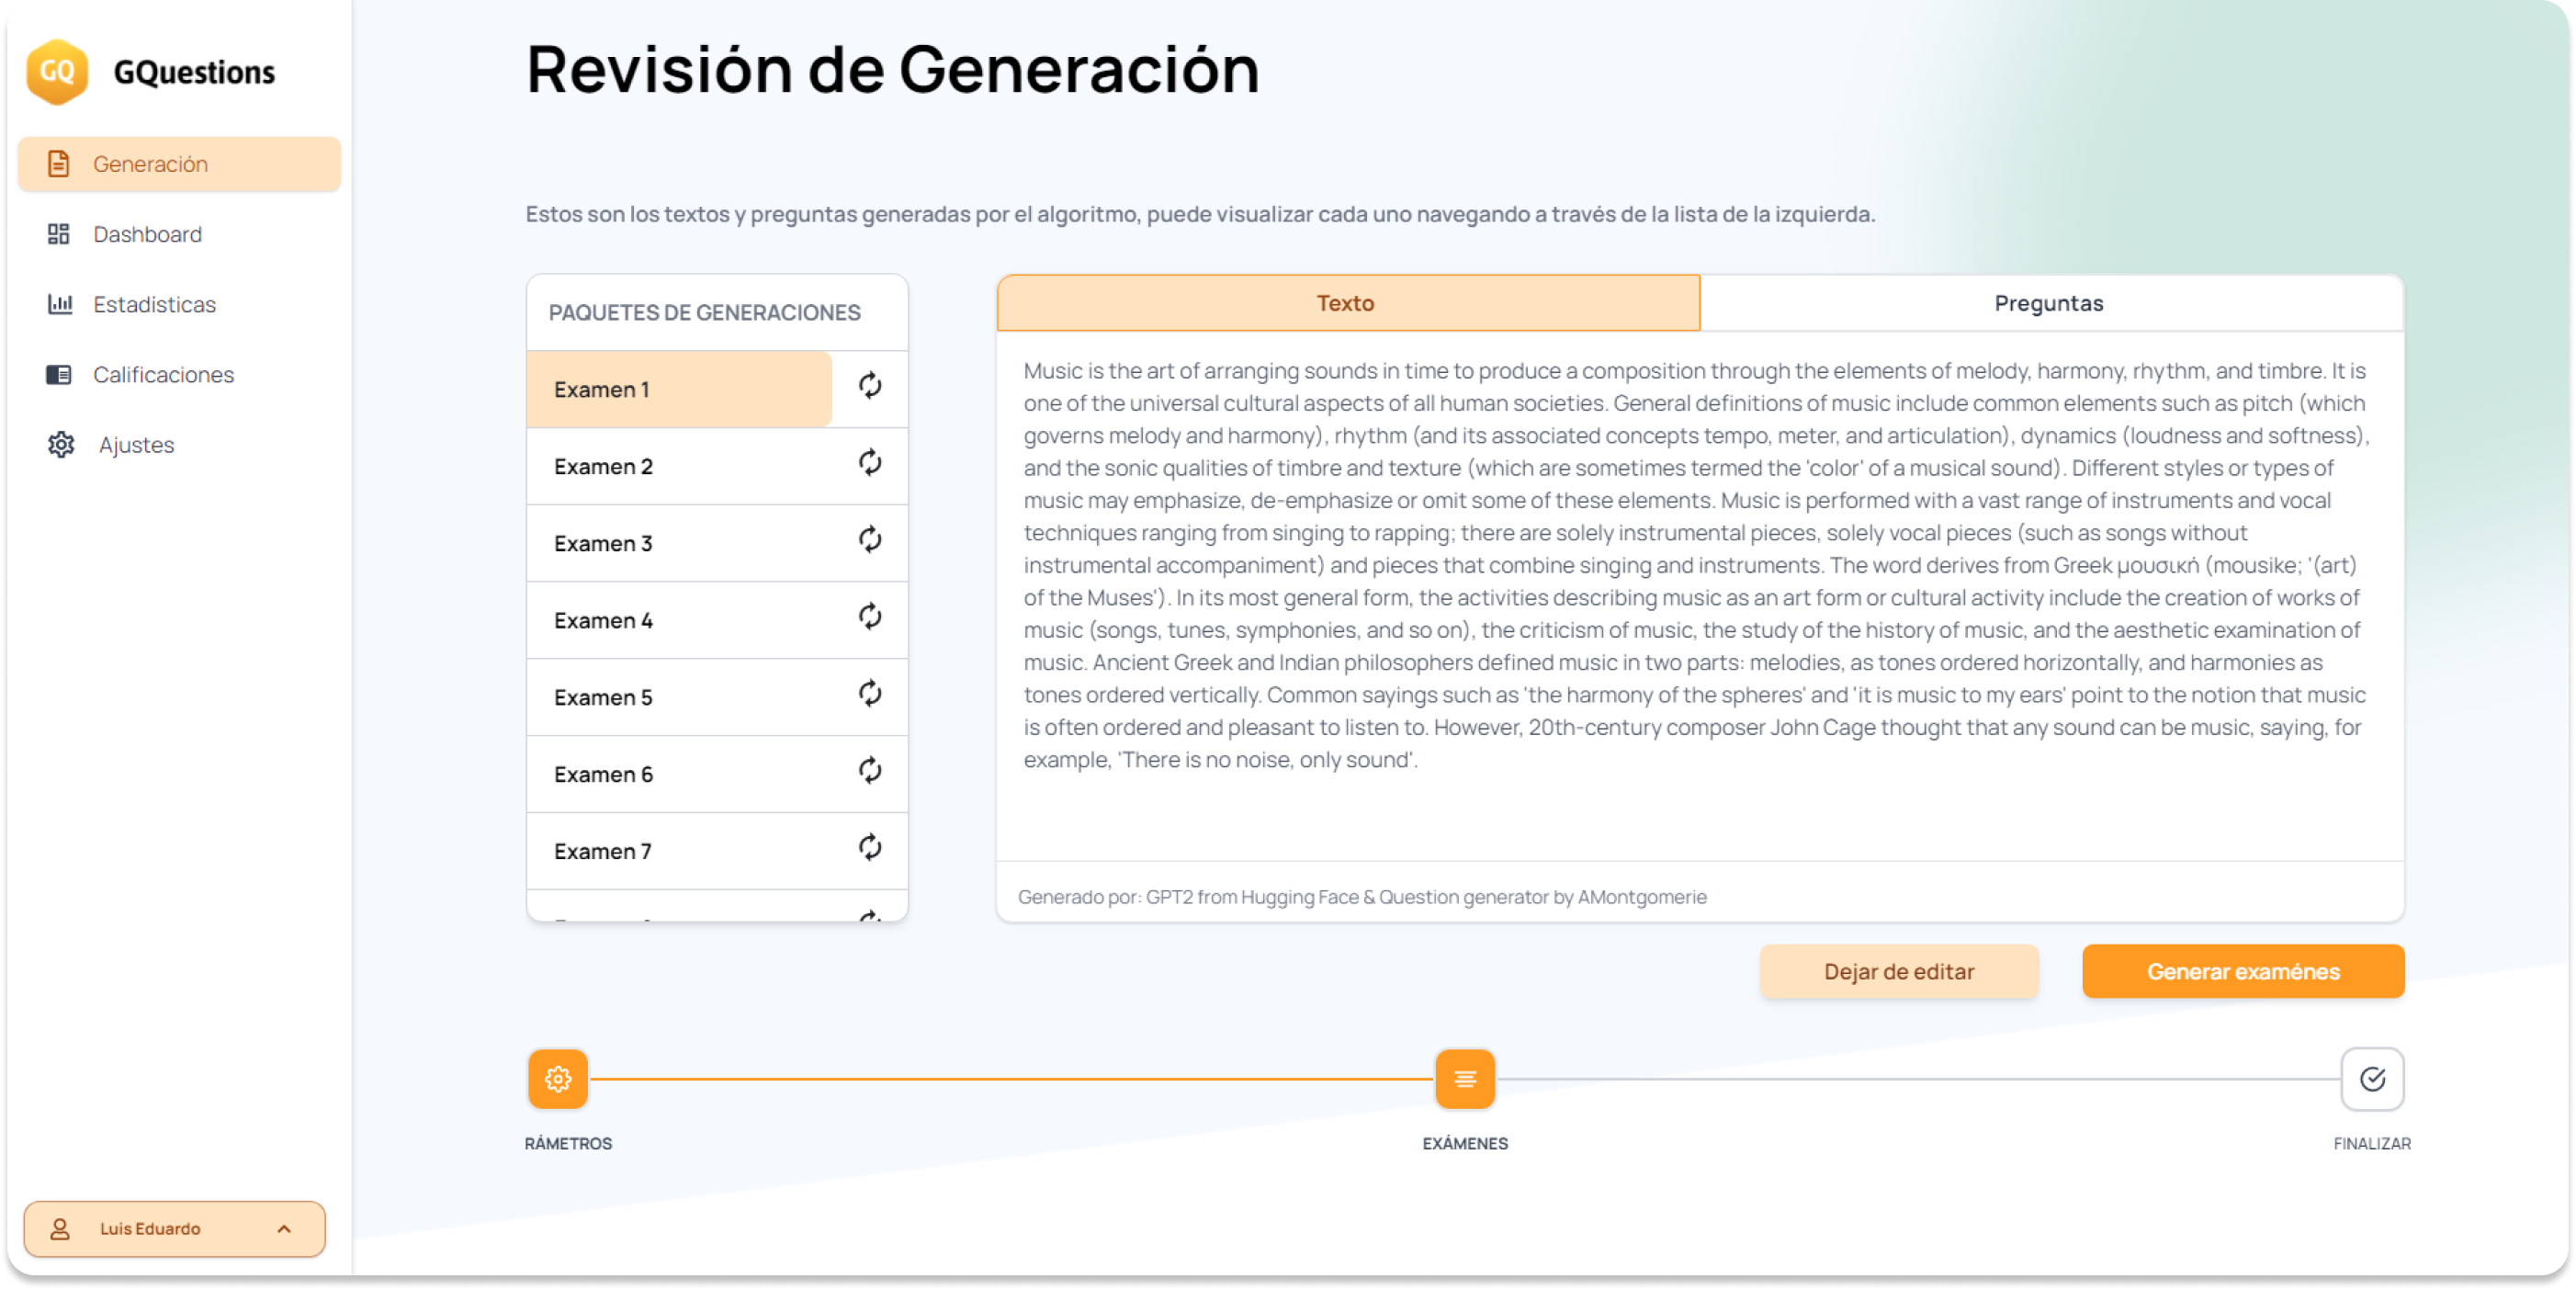
\includegraphics[width=6.4in,height=3.3in]{Images/ui_docente_revision_generacion.png}
	    \caption{UI Revisión de generación - docente}
	    Fuente: Elaboración propia
        \label{fig:section}
	\end{Center}
    \end{figure}
    
    %--------------------- Submódulo de conf exámenes ---------------------
    \subsubsection{Submódulo Configuración conjunto de exámenes}
    \begin{justify}
    Este submódulo representa el tercer y último paso de la generación, permite configurar el conjunto de exámenes en cuanto a disposición del mismo para los estudiantes, con campos como fecha y hora de inicio y finalización, contraseña, duración y nombre del conjunto de exámenes.
    
    \begin{figure}[H]
	\begin{Center}
		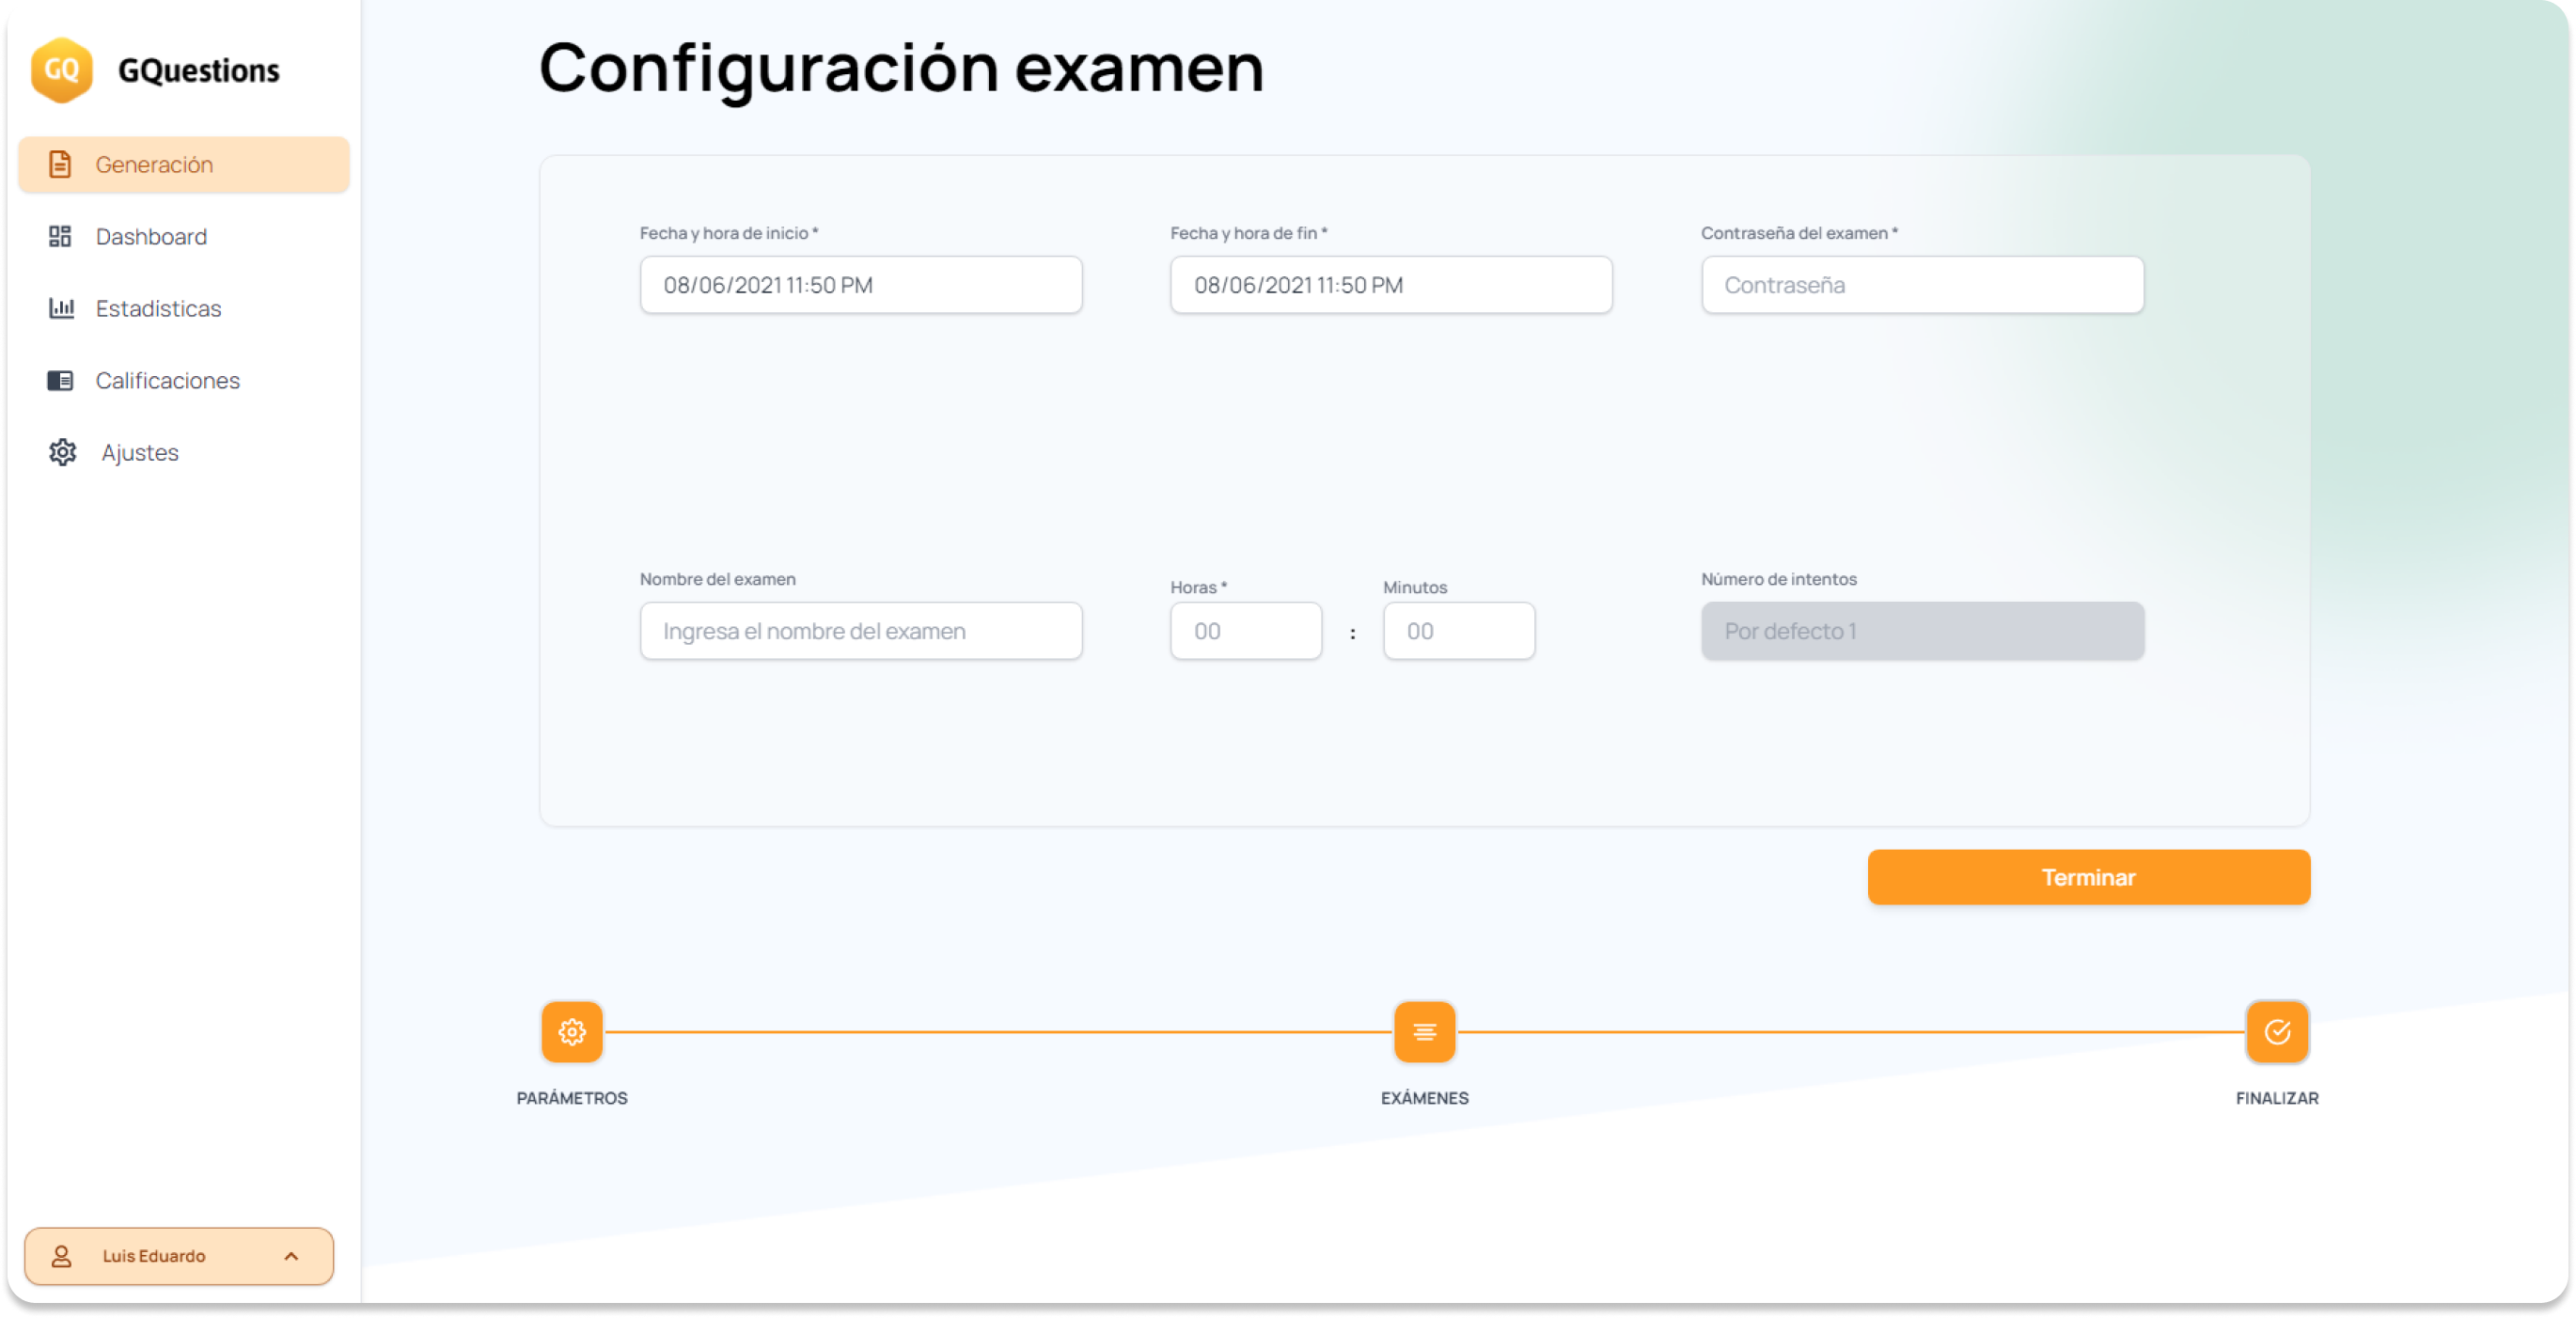
\includegraphics[width=6.4in,height=3.3in]{Images/ui_docente_conf_examen.png}
	    \caption{UI Configuración examen - docente}
	    Fuente: Elaboración propia
        \label{fig:section}
	\end{Center}
    \end{figure}
    \end{justify}
    
    %--------------------- Módulo de examen ---------------------
    \subsection{Módulo Examen}
    \begin{justify}
    Este módulo permite a los estudiantes responder los exámenes generados por el docente, accediendo a ellos por medio de un enlace y contraseña, además, se realiza la calificación del examen por parte del sistema. La interfaz gráfica de este módulo es muy similar a la del submódulo de la sección revisión de examen 5.2.6.2.
    \end{justify}
    
    %--------------------- Módulo de estadísticas ---------------------
    \subsection{Módulo Estadísticas}
    \begin{justify}
    Este módulo muestra la información del usuario relacionada a las generaciones, se puede visualizar el total de número de generaciones, exámenes, textos y preguntas generadas, además, se puede visualizar el número de generaciones por mes. 
    \end{justify}
    
    \begin{figure}[H]
	\begin{Center}
		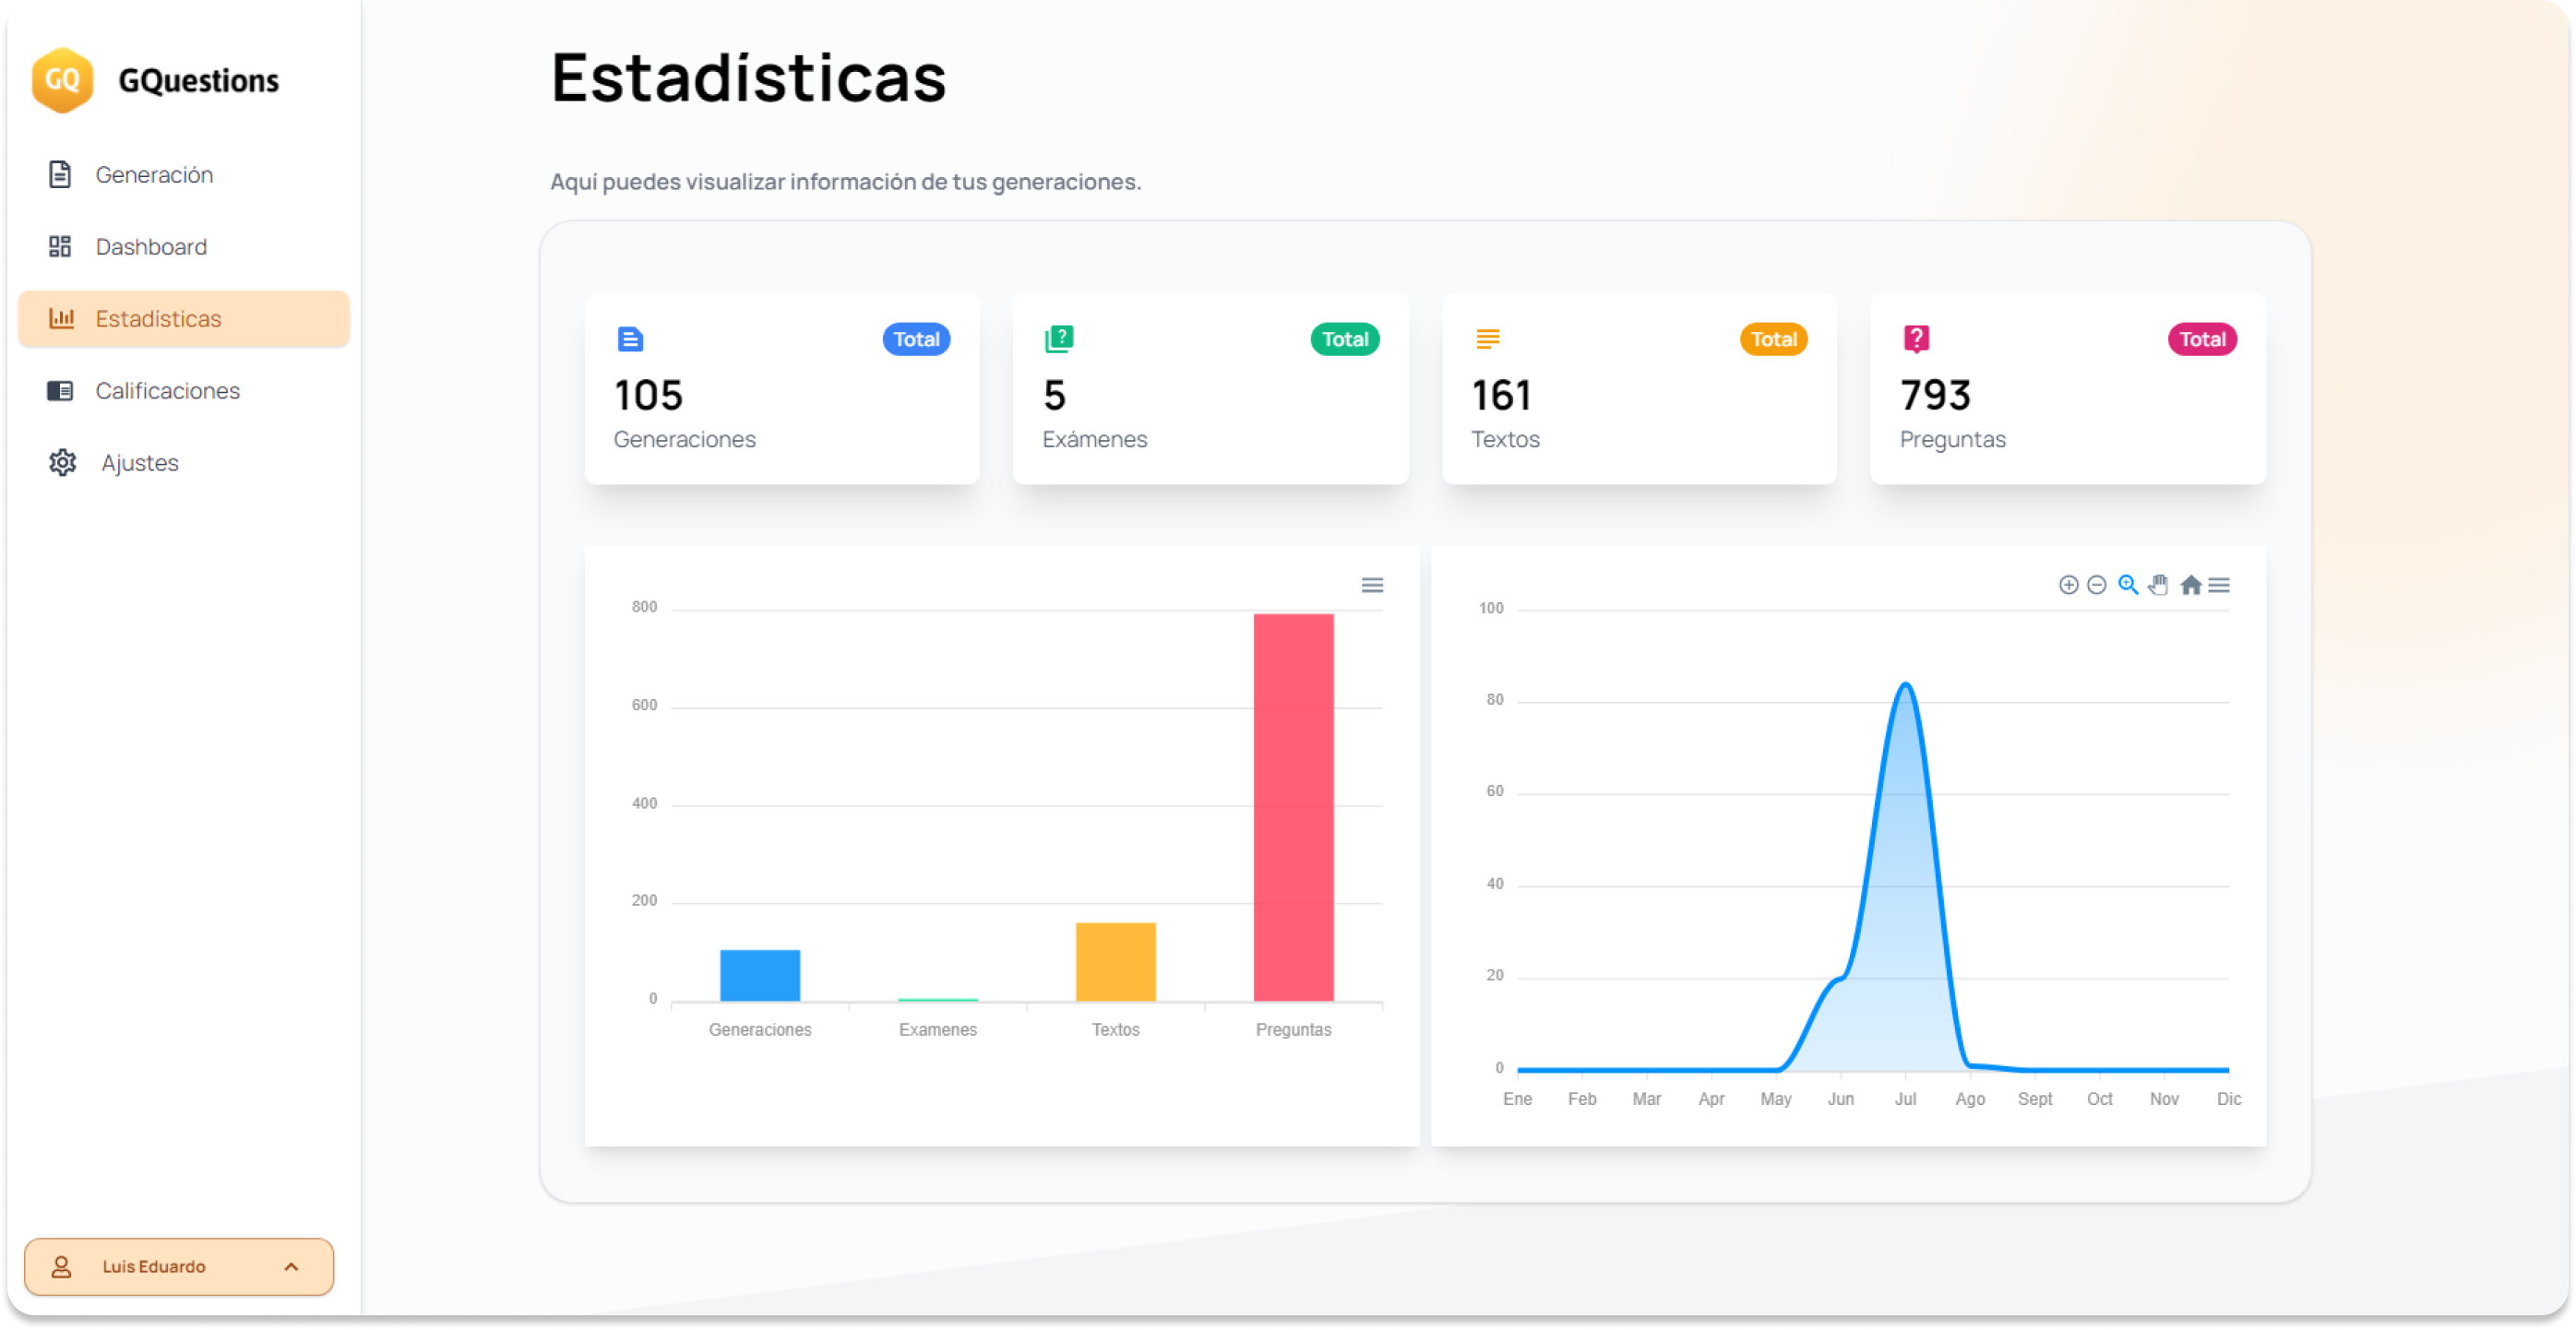
\includegraphics[width=6.4in,height=3.3in]{Images/ui_docente_estadisticas.png}
	    \caption{UI Estadísticias - docente}
	    Fuente: Elaboración propia
        \label{fig:section}
	\end{Center}
    \end{figure}
    
    %--------------------- Módulo de calificaciones ---------------------
    \subsection{Módulo Calificaciones}
    \begin{justify}
    Este módulo permite visualizar el listado de exámenes que ha aplicado el docente, contiene varios submódulos que permiten revisar las calificaciones de los estudiantes. 
    \end{justify}
    
    \begin{figure}[H]
	\begin{Center}
		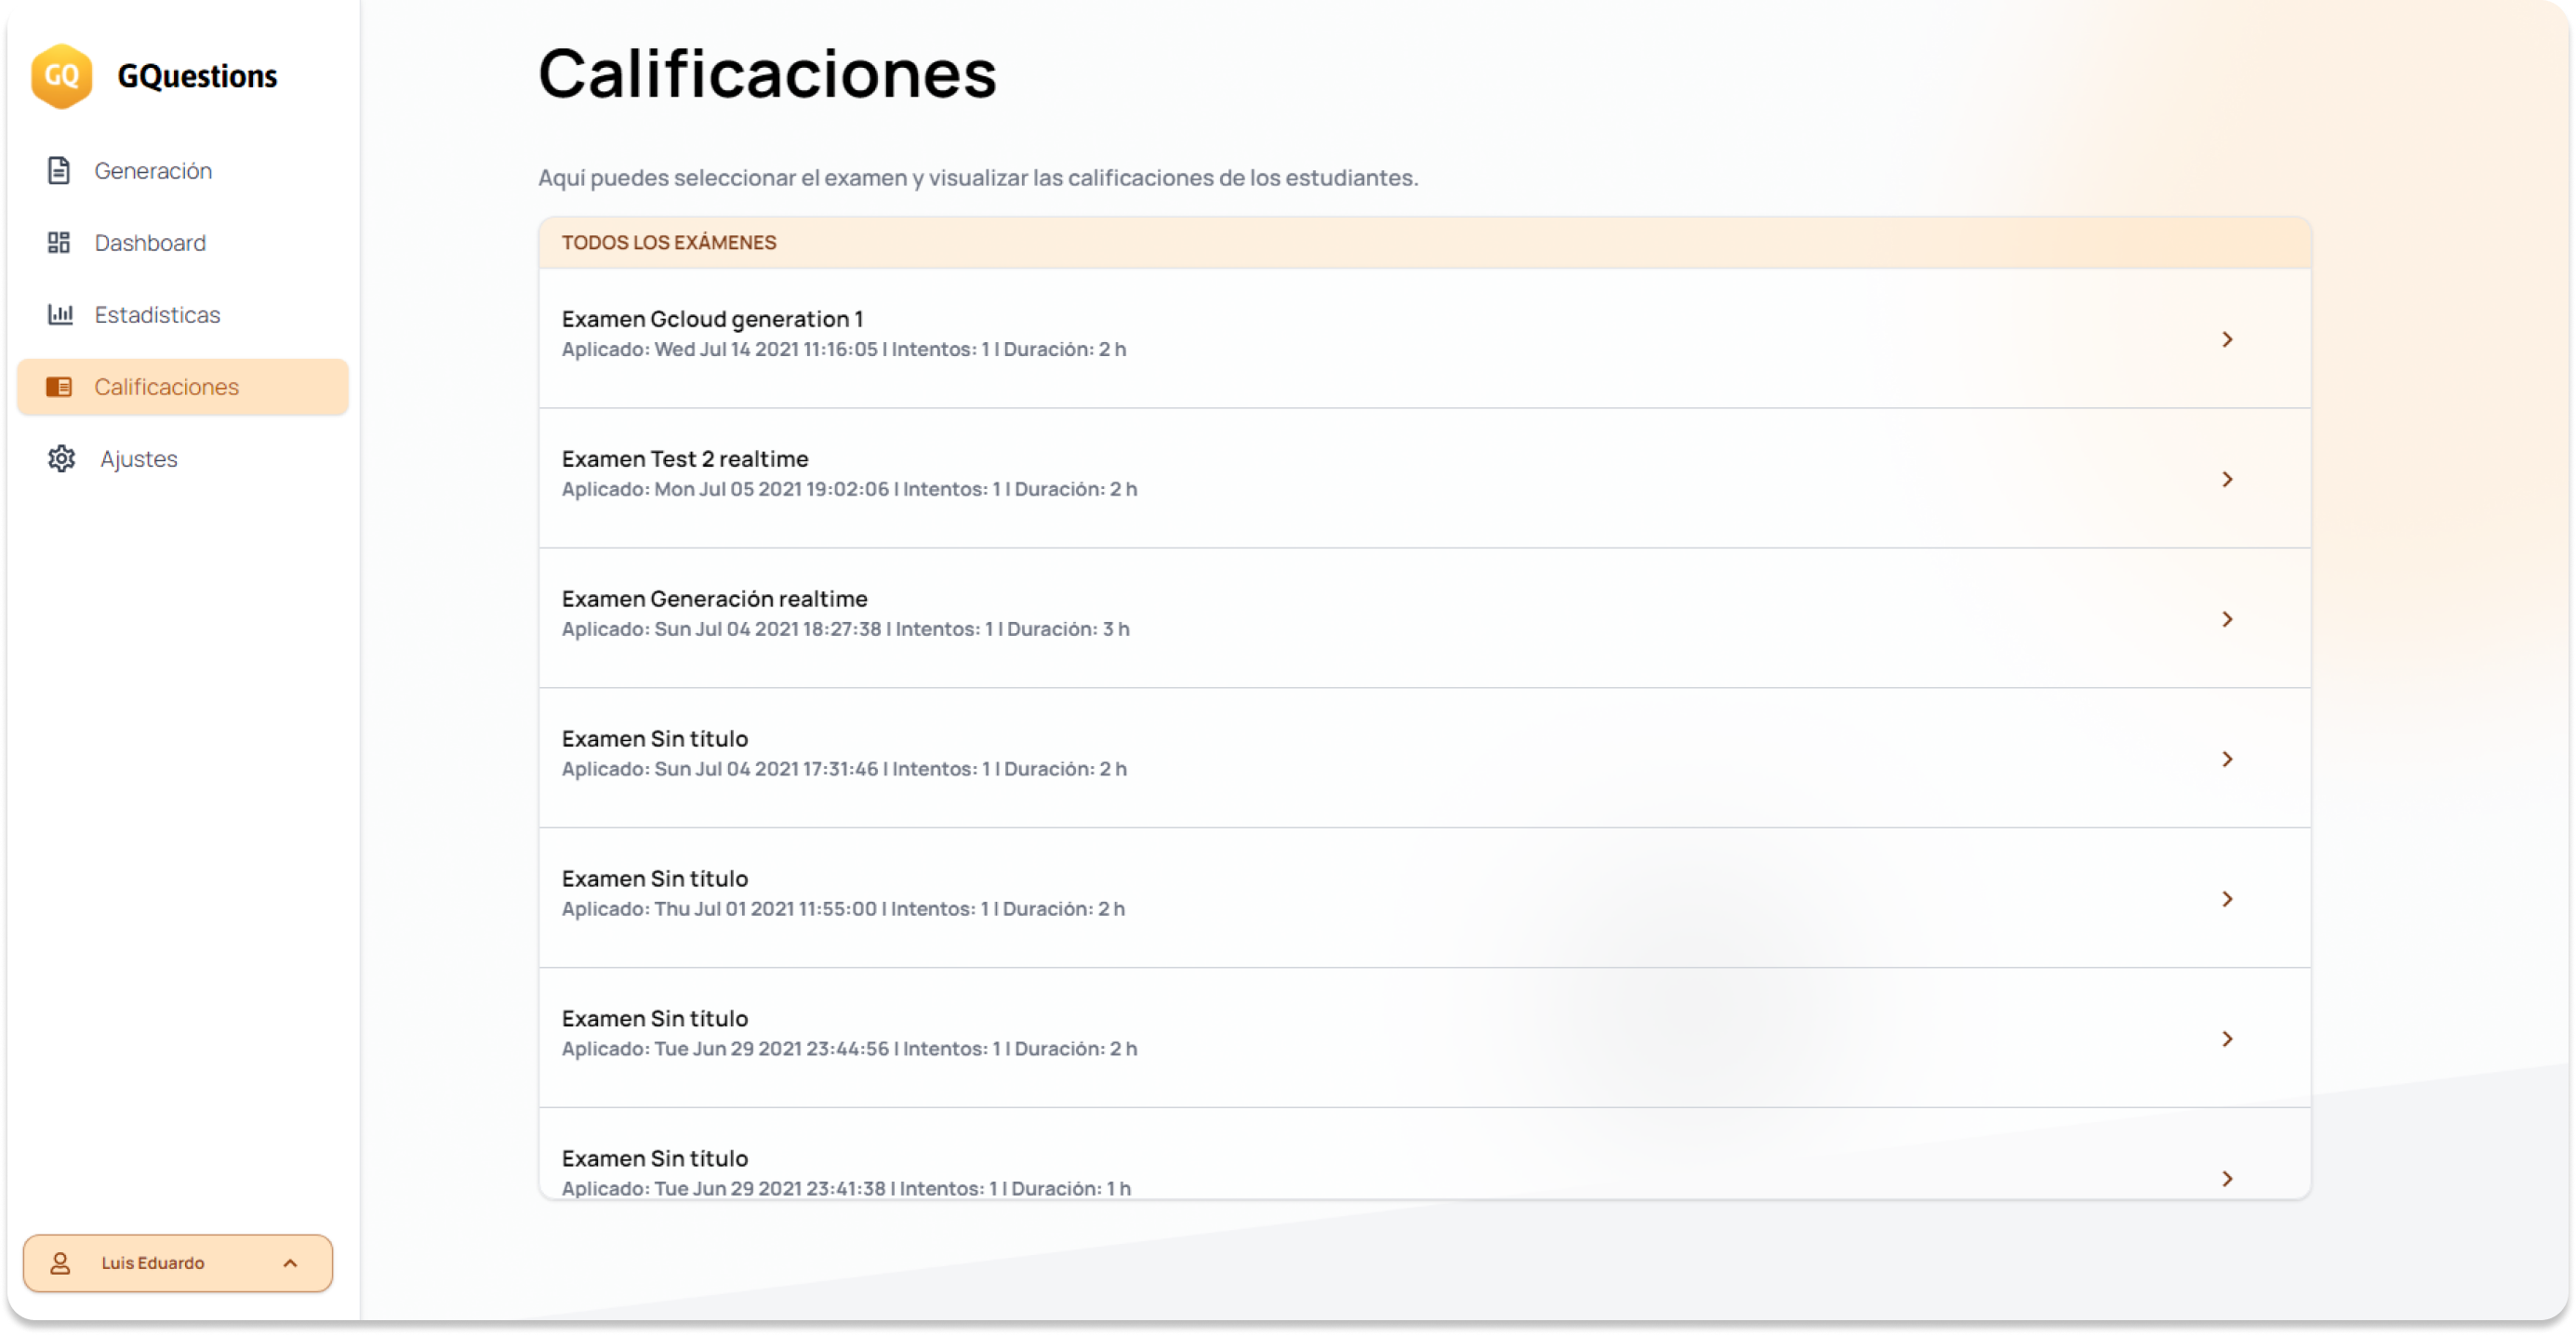
\includegraphics[width=6.4in,height=3.3in]{Images/ui_docente_calificaciones.png}
	    \caption{UI Calificaciones}
	    Fuente: Elaboración propia
        \label{fig:section}
	\end{Center}
    \end{figure}
    
    \subsubsection{Submódulo Lista de calificaciones}
    \begin{justify}
    Este submódulo permite visualizar un listado de los estudiantes junto con las las calificaciones correspondientes, el docente puede modificar la calificación en caso de ser necesario.
    \end{justify}

    \begin{figure}[H]
	\begin{Center}
		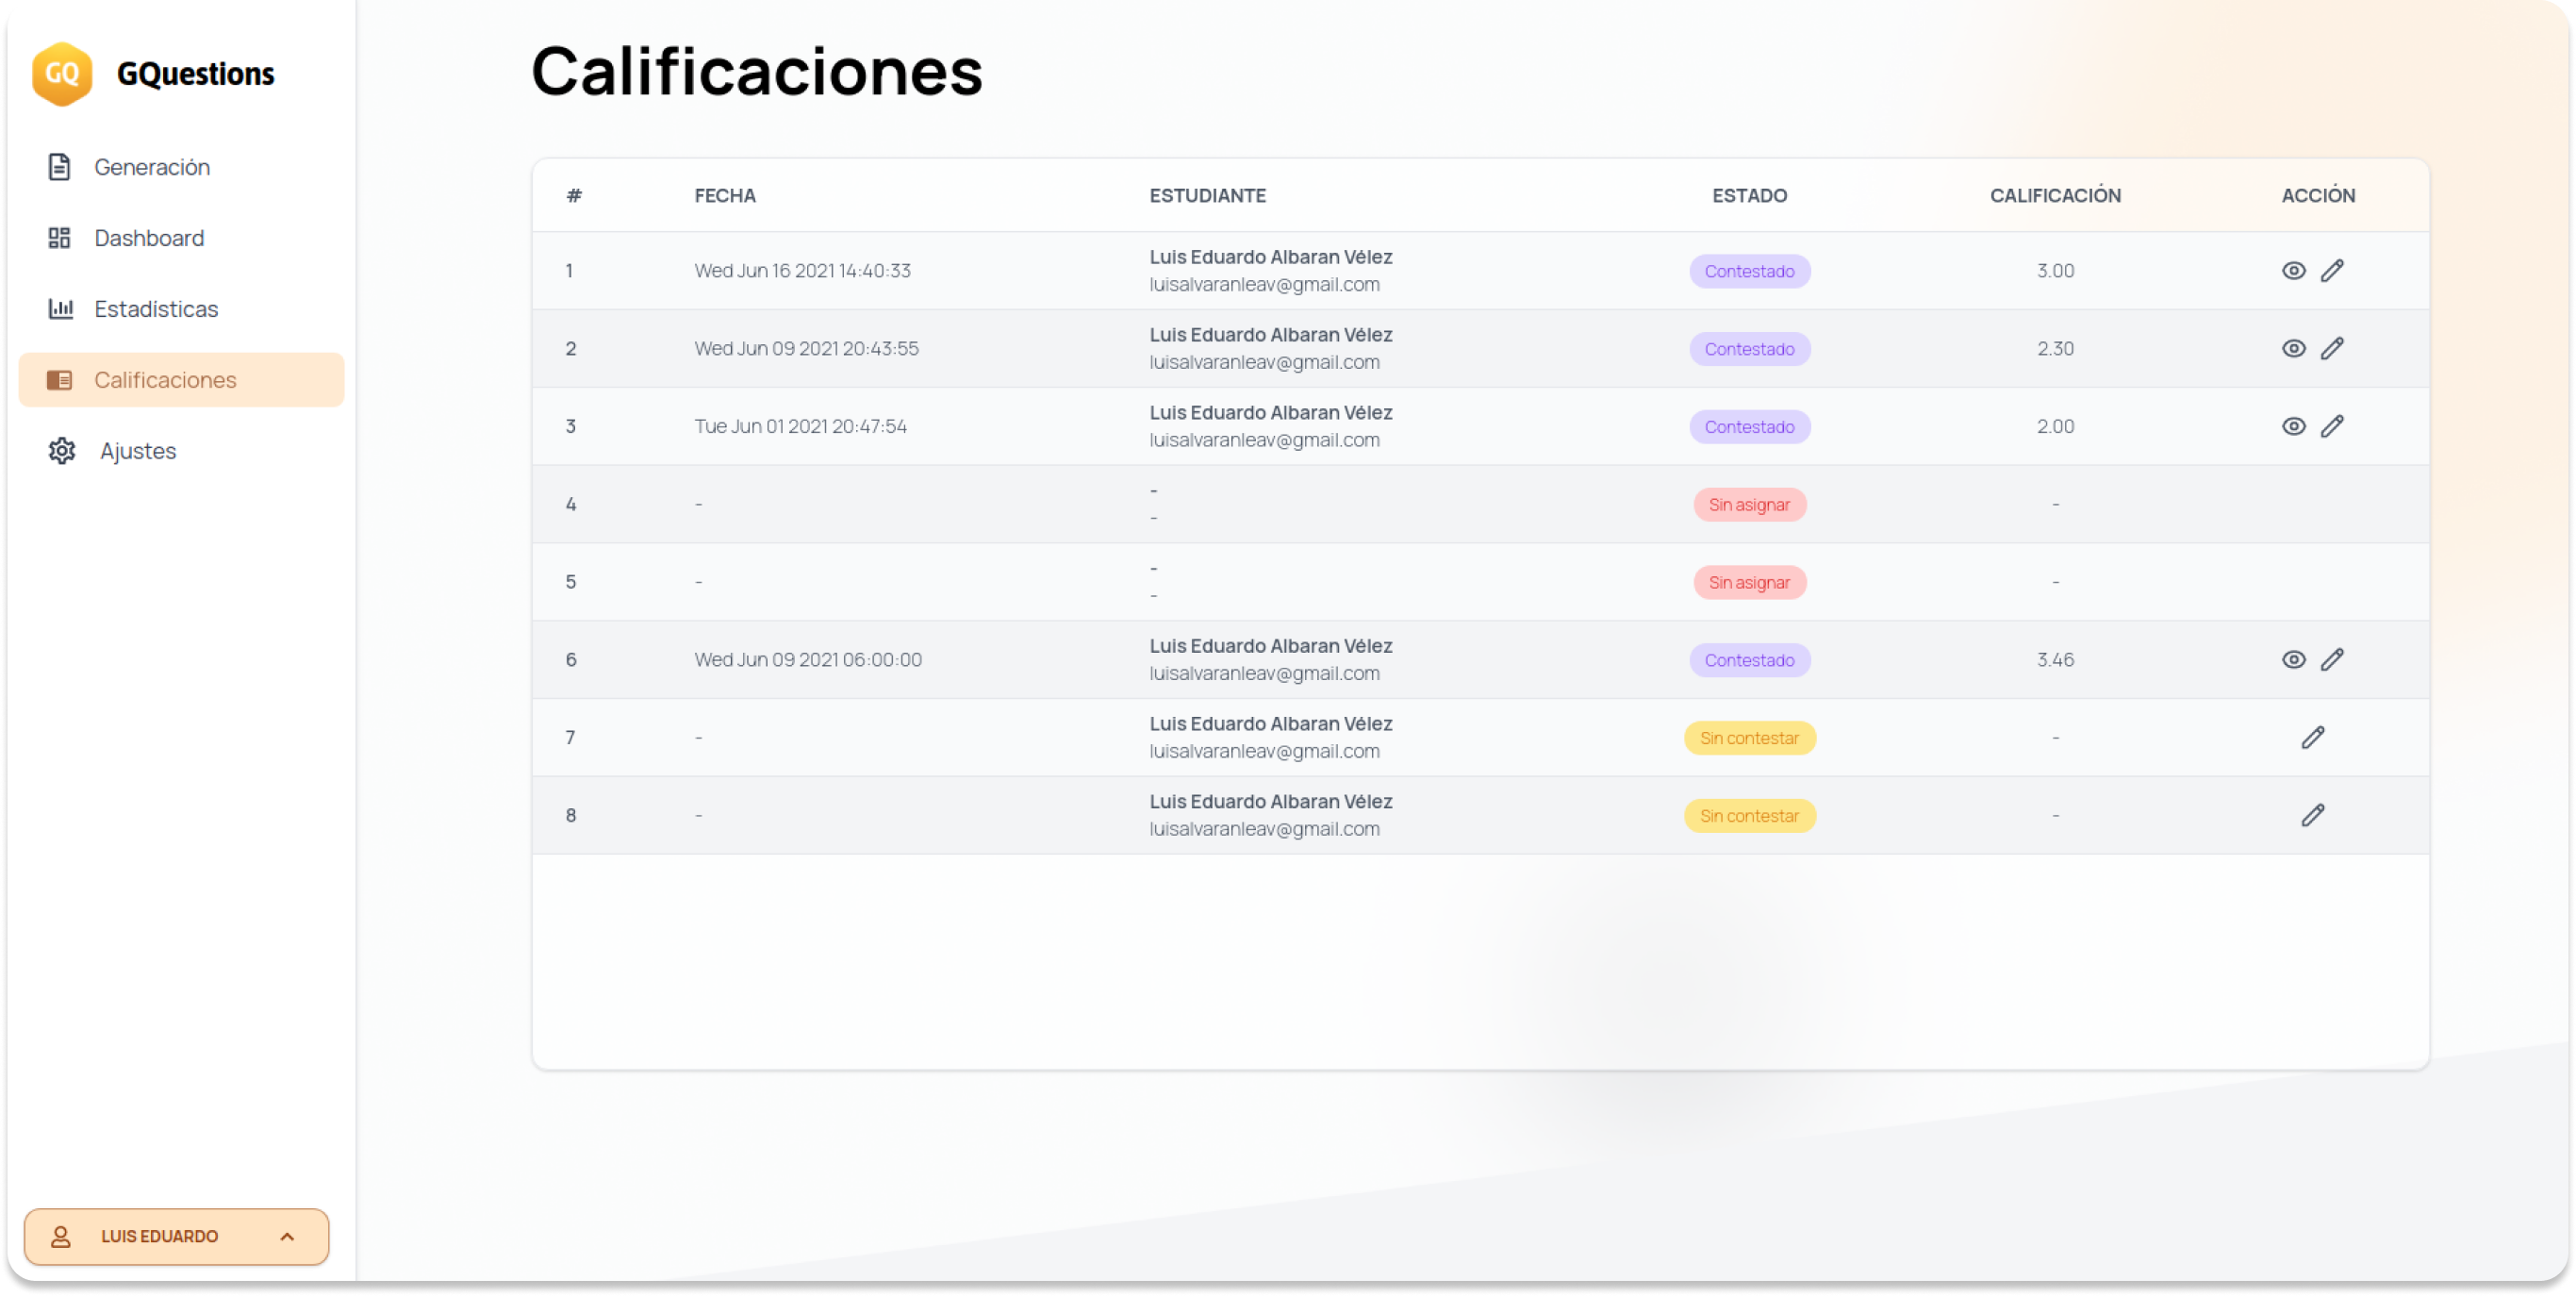
\includegraphics[width=6.4in,height=3.3in]{Images/ui_docente_listado_calificaciones.png}
	    \caption{UI Listado de calificaciones}
	    Fuente: Elaboración propia
        \label{fig:section}
	\end{Center}
    \end{figure}
    
    \subsubsection{Submódulo Revisión de examen}
    \begin{justify}
    Este submódulo permite revisar el examen resuelto, visualizar el texto base, las preguntas, las respuestas del estudiante, las respuestas correctas y la calificación de cada pregunta y global.
    \end{justify}

    \begin{figure}[H]
	\begin{Center}
		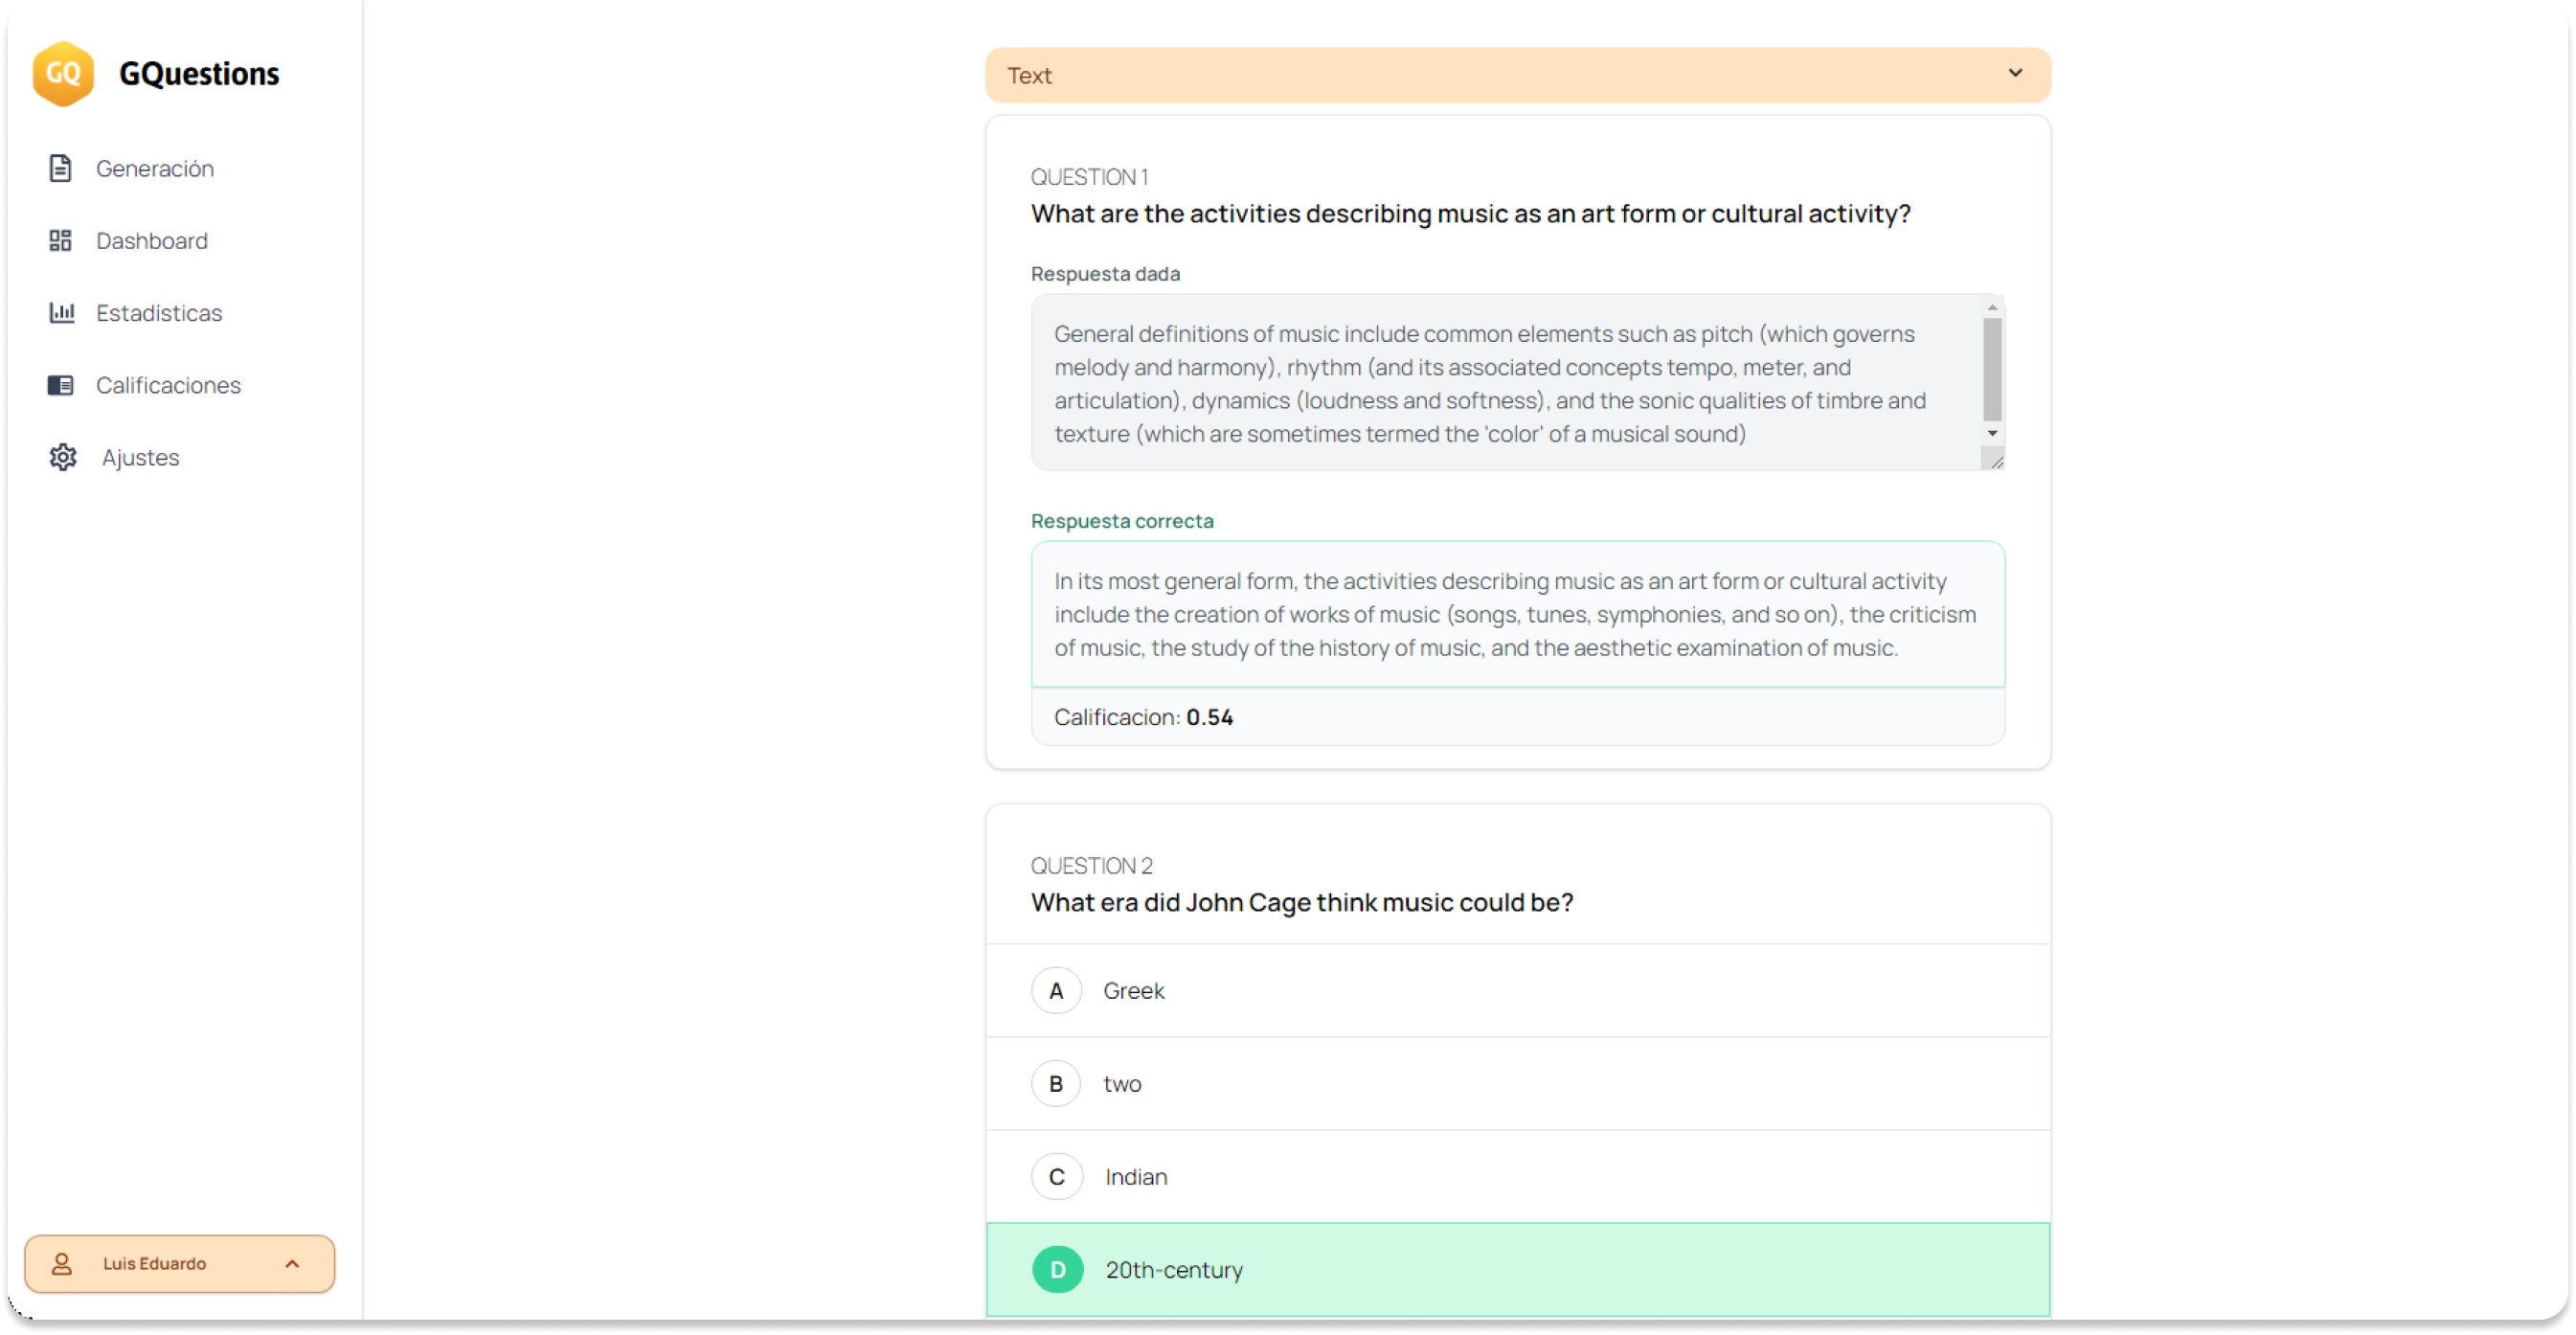
\includegraphics[width=6.4in,height=3.3in]{Images/ui_revision_examen.png}
	    \caption{UI Revisión de examen}
	    Fuente: Elaboración propia
        \label{fig:section}
	\end{Center}
    \end{figure}
    
\end{document}